\section{Basics of Convex Analysis}
In order to understand stochastic gradient descent we need to understand deterministic gradient descent. Gradient descent is an algorithm that is part of a family of algorithms called descent methods which are mostly applicable to unconstrained minimization problems. When dealing with unconstrained problems, an important assumption is the convexity of the objective function. To understand convexity, we need to understand the notions of affine sets and convex sets. Additionally, further definitions and regularity conditions require examination. These concepts are important because the convexity assumption plays a crucial role in the convergence properties of deterministic and stochastic gradient descent. The primary reference for this section, and much of the mathematical framework that will be used throughout this thesis, is 'Convex Optimization' by Stephen Boyd and Lieven Vandenberghe \cite{boyd2004convex}.
\subsection{Convexity}
\begin{definition}
Suppose $x_{1},x_{2} \in \mathbb{R}^{n}$ with $x_{1} \neq x_{2}$. Points of the form $y = \theta x_{1} + (1-\theta) x_{2},$ where $\theta \in \mathbb{R}$, form the $\textit{line}$ passing through $x_{1}$ and $x_{2}$. The parameter value $\theta = 0$ corresponds to $y = x_{2}$ and the value $\theta = 1$ corresponds to $y = x_{1}$. The set $[x_{1},x_{2}] = \{\theta x_{1} + (1-\theta) x_{2}: \theta \in [0,1]\}$ is called the (closed) \textit{line segment} between $x_{1}$ and $x_{2}$. In other words, the line starts at $x_{1}$ and ends at $x_{2}.$
\end{definition}

\begin{definition}
(\cite[21]{boyd2004convex})
A set $C\subseteq\mathbb{R}^{n}$ is \textit{affine} if the line through any two distinct points in \textit{C} lies in \textit{C}. In other words, if for any $x_{1}, x_{2} \in C$ and $\theta \in \mathbb{R}$, we have $\theta x_{1} + (1-\theta) x_{2} \in C$.
\end{definition}

\begin{definition}
(\cite[23]{boyd2004convex})
A set $C \subseteq \mathbb{R}^{n}$ is \textit{convex} if the line segment between any two points in \textit{C} lies in \textit{C}, In other words, if for any $x_{1}, x_{2}$ $\in C$ and $\theta\in [0,1]$, we have $\theta x_{1} + (1-\theta) x_{2} \in C.$
\end{definition}
\vspace*{0pt}
\begin{figure}[h!]
    \centering
        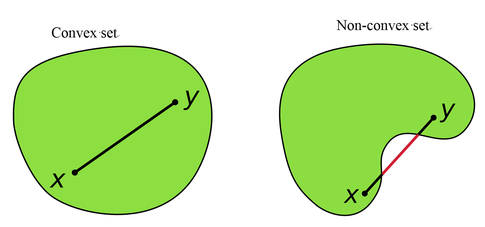
\includegraphics[width=0.4\textwidth]{Pictures/Convex ex.png}
    \caption{Example of a convex and non-convex set}
    \label{fig:conv-nonconv}
\end{figure}

\begin{definition}
(\cite[36]{boyd2004convex})
A function $f:C\subseteq\mathbb{R}^{n} \longrightarrow \mathbb{R}^m$ is \textit{affine} if it is a sum of a linear function and a constant, in other words, if it has a form $f(x) = Ax + b$, where $A \in \mathbb{R}^{m \times n}$ and $b \in \mathbb{R}^m$.
\end{definition}

\begin{definition}\label{definition.2.4}
(\cite[67]{boyd2004convex})
A function $f: C\subseteq\mathbb{R}^{n} \longrightarrow \mathbb{R}$ is convex if $C$ is  convex, and
\begin{equation*}\label{eq:4}\tag{3.1.1}
\begin{aligned}
    &f(\theta x + (1-\theta) y) \leq \theta f(x) + (1-\theta) f(y)
\end{aligned}
\end{equation*}
for all $x,y \in C$, and $\theta\in [0,1].$
\end{definition}

\begin{proposition}\label{compaf}
\textnormal{(\cite[79]{boyd2004convex})}
Suppose $f: \mathbb{R}^{n} \longrightarrow \mathbb{R}, \text{ } A \in \mathbb{R}^{m\times n},$ and $b \in \mathbb{R}^{m}.$ Define $g: \mathbb{R}^{m} \longrightarrow \mathbb{R}$ by $$g(x)=f(Ax+b).$$ Then if $f$ is convex, so is $g$.
\end{proposition}
\begin{proof}
Let $f: \mathbb{R}^{n} \longrightarrow \mathbb{R}$ be convex. Fix $A \in \mathbb{R}^{m\times n}, \text{ }b \in \mathbb{R}^{m}, \text{ }x,y \in \mathbb{R}^{n}$ and $\theta \in [0,1].$ Then
\begin{align*}
g(\theta x + (1-\theta)y) &= f(A(\theta x + (1-\theta)y) + b)\\
&= f(\theta(Ax - Ay) + Ay + b)\\
&= f(\theta(Ax + b) + (1 - \theta)(Ay+b))\\
&\leq \theta f(Ax + b) + (1-\theta) f(Ay + b)\\
&= \theta g(x) + (1-\theta)g(y).
\end{align*}
$A,$ $b,$ $x,y$ and $\theta$ are fixed. So the inequality holds for all $A \in \mathbb{R}^{m\times n}, b \in \mathbb{R}^{m}, \text{ } x,y \in \mathbb{R}^{n}$ and $\theta \in [0.1].$ Hence, $g$ is convex. Moreover, $f$ is an arbitrary convex function. So the inequality holds for all convex functions. We conclude that the composition of a convex function with an affine function is convex.
\end{proof}
\subsection{Gradient and Optimality}
\begin{definition}[Gradient]\label{gradient}
If $f:\mathbb{R}^{n}\longrightarrow\mathbb{R}$ is differentiable along each axis, we denote 
\begin{equation*}\tag{3.2.1}
\begin{aligned}
    &\nabla f(x) \overset{def.}{=} \left(\frac{\partial f(x)}{\partial x_{1}},\ldots,\frac{\partial f(x)}{\partial x_{d}}\right)^{T} \in \mathbb{R}^{n}
\end{aligned}\
\end{equation*}
as the gradient vector, so that $\nabla f:\mathbb{R}^{n}\longrightarrow \mathbb{R}^{n}$ is a vector field.
\end{definition}
\begin{lemma}[First-order conditions]\label{lemma.2.1}
\textnormal{(\cite[69]{boyd2004convex})}
Suppose $f:\mathbb{R}^{n}\rightarrow\mathbb{R}$ is differentiable. In other words, $\nabla f$ exists at each point in $\mathbb{R}^{n}$. Then \textit{f} is convex if and only if
\begin{equation*}\label{eq:5}\tag{3.2.2}
\begin{aligned}
    &f(y) \geq f(x) + \nabla f(x)^{T}(y-x)
\end{aligned}
\end{equation*}
holds for all $x,y \in \mathbb{R}^{n}$.
\end{lemma}
The affine function $y\mapsto f(x)+\nabla f(x)^{T}(y-x)$ is, of course, the first-order Taylor approximation of $f$ near $x.$ Lemma \ref{lemma.2.1} contains an if and only if statement which states that for convex functions, the first-order Taylor approximation is always a \textit{global under estimator} for the function and that the converse is also true. In the context of optimization, finding the minimum value of a function requires identifying the point at which the function attains its lowest value. Setting the gradient to zero serves as a means of locating an optimal solution, a point of inflection where the rate of change of the function is zero and the function is neither increasing nor decreasing. 
\begin{proposition}\label{eq:local_conv}
\textnormal{(\cite[7]{coursenotesML})}
If $f:\mathbb{R}^{n}\longrightarrow\mathbb{R}$ attains a local minimum at $x^{*},$ then $\nabla f(x^{*}) = 0.$
\end{proposition}
\begin{proof}
One has for $\epsilon$ small enough and $u$ fixed
$$f(x^{*}) \leq f(x^{*} + \epsilon u) = f(x^{*}) + \epsilon \langle \nabla f(x^{*}),\text{ }u\rangle + o(\epsilon) \implies \langle \nabla f(x^{*}),\text{ }u\rangle \geq o(1) \implies \langle \nabla f(x^{*}),\text{ }u\rangle \geq 0.$$ So applying this for $u$ and $-u$ in the previous equation shows that $\langle \nabla f(x^{*}),\text{ }u\rangle = 0$ for all $u$, and hence $\nabla f(x^{*}) = 0.$
\end{proof}
\begin{proposition}\textnormal{(\cite[7]{coursenotesML})}\label{eq:argmin_conv}
Let $f:\mathbb{R}^{n}\longrightarrow\mathbb{R}$ be a function.
\begin{enumerate}
    \item If $f$ is convex and attains a local minimum at $x^{*}$, then this local minimum is also a global minimum.
    \item If $f$ is differentiable and convex, then $x^{*} \in \underset{x}{\textnormal{argmin}}f(x) \iff \nabla f(x^{*}) = 0$.
\end{enumerate}
\end{proposition}
\begin{proof}
\textbf{First bullet point:}
Let $x \in \mathbb{R}^n$ be fixed. Then there exists $0 < \theta < 1$ small enough such that $\theta x + (1-\theta)x^{*}$ is close enough to $x^{*}$, and since it is a local minimizer, we have:
\[
f(x^{*}) \leq f(\theta x + (1-\theta)x^{*}) \leq \theta f(x) + (1-\theta) f(x^{*}) \implies f(x^{*}) \leq f(x).
\]
Now, $x \in \mathbb{R}^n$ is fixed, so this inequality holds for all $x \in \mathbb{R}^n$, thus $x^{*}$ is a global minimum.

\textbf{Second bullet point:}
The '$\Rightarrow$' implication is proven in Proposition \ref{eq:local_conv}. Fix $x,x^{*}\in\mathbb{R}^{n}$ and suppose that $\nabla f(x^{*}) = 0$. As stated in Lemma \ref{lemma.2.1}, $f(x)$ is bounded below by its tangent, we have:
\[
f(x) \geq f(x^{*}) + \langle \nabla f(x^{*}),\, x - x^{*}\rangle = f(x^{*}).
\]
$x,x^{*}\in\mathbb{R}^{n}$ are fixed, so $f(x)\geq f(x^{*})$ for all $x,x^{*}\in\mathbb{R}^{n}$ with $\nabla f(x^{*})=0.$
\end{proof}
The last inequality shows that $x^{*}$ is a global minimizer of the function $f$. Hence, if \textit{f} is differentiable and convex, a necessary and sufficient condition for a point $x^{*}$ to be optimal is given by: $\nabla f(x^{*}) = 0.$ 
One can strengthen the convexity condition from Definition \ref{definition.2.4} and impose that the inequality is strict for $f:\mathbb{R}^{n}\longrightarrow\mathbb{R}.$ In this case, $f$ is called strictly convex. 
\begin{definition}\label{strict_convexity}
A function $f: C\subseteq\mathbb{R}^{n} \longrightarrow \mathbb{R}$ is strictly convex if $C$ is a convex set, and
\begin{equation*}\label{eq:strict_conv}\tag{3.2.3}
\begin{aligned}
    &f(\theta x + (1-\theta) y) < \theta f(x) + (1-\theta) f(y)
\end{aligned}
\end{equation*}
for all $x,y \in C$ with $x\neq y$, and $\theta\in (0,1)$.
\end{definition}    
Proposition \ref{strict_conv_imp_unique} provides a valuable result for strictly convex functions.
\begin{proposition}\label{strict_conv_imp_unique}
If $f:C\subseteq\mathbb{R}^{n}\longrightarrow\mathbb{R}$ is strictly convex, and $x^{*}\in\underset{x}{\textnormal{argmin}}f(x)$ exists, it is unique.
\end{proposition}
\begin{proof}
Let $f:C\subseteq\mathbb{R}^{n}\longrightarrow\mathbb{R}$ be strictly convex. Suppose that there exists $x_{1}^{*}, x_{2}^{*}\in C$ with $x_{1}^{*}\neq x_{2}^{*}$ such that $x_{1}^{*}, x_{2}^{*} \in \underset{x}{\textnormal{argmin}}f(x).$ We choose $\theta=\frac{1}{2}.$ Then by strict convexity, 
\begin{comment}
\begin{equation*}
f(x_{1}^{*}) = f(\frac{x_{1}^{*}+x_{2}^{*}}{2}) < \frac{1}{2} f(x_{1}^{*}) + \frac{1}{2} f(x_{2}^{*}) = f(x_{1}^{*}) \hspace{0.4cm} \text{{\Large \Lightning}}
\end{equation*}
\end{comment}
We reach a contradiction. Thus, if minimizers for strictly convex functions exist, they are unique. 
\end{proof}
Lemma \ref{lemma.2.1} will especially prove to be useful in the convergence analysis of descent methods. In many situations neither Definition \ref{definition.2.4} nor Lemma \ref{lemma.2.1} are used to check the convexity of a function. Additional conditions called the second-order conditions are often used to check convexity of a function. Before going over the second-order conditions, we first need the notions of the Hessian and positive semidefiniteness. 
\begin{definition}[Hessian]
(\cite[748]{adams2013calculus})
Suppose $f: \mathbb{R}^{n} \longrightarrow \mathbb{R}$ is a function with the property that all second-order partial derivatives of $f$ exist, then the Hessian of $f$ is an $n \times n$ matrix and is given by:
\begin{equation*}\tag{3.2.4}
\begin{aligned}
\mathcal{H}_{f} =
& \begin{bmatrix}
    f_{11}(x) & f_{12}(x) & \cdots & f_{1d}(x) \\
    f_{21}(x) & f_{22}(x) & \cdots & f_{2d}(x) \\
    \vdots    & \vdots    & \ddots & \vdots    \\
    f_{d1}(x) & f_{d2}(x) & \cdots & f_{dd}(x)
  \end{bmatrix}
  \hspace{0.2cm}
  \text{where}\text{ } f_{ij} = \frac{\partial^{2}f}{\partial x_{i}\partial x_{j}}
\end{aligned}
\end{equation*}
\end{definition}
\begin{definition}[Positive semidefiniteness]\label{posdef}
(\cite{doi:https://doi.org/10.1002/9780470173862.app3})
Suppose that $\mathcal{V}$ is an $n \times n$ symmetric matrix, i.e., $\mathcal{V}=\mathcal{V}^{T}$, then $\mathcal{V}$ is said to be positive semidefinite if 
\begin{equation*}\label{eq:6}\tag{3.2.5}
\begin{aligned}
    &x^{T} \mathcal{V} x \geq 0 
\end{aligned}
\end{equation*}
for all $x \in \mathbb{R}^{n}$. Notation: $\mathcal{V} \succeq 0.$
\end{definition}
\begin{lemma}[Second-order conditions]\label{second-ord-cond}
\textnormal{(\cite[71]{boyd2004convex})}
Suppose $f:\mathbb{R}^{n}\longrightarrow\mathbb{R}$ is twice differentiable, that is, its Hessian or second derivative $\nabla^{2}f$ exists at each point in $\mathbb{R}^{n}$. Then f is convex if and only if its Hessian is positive semidefinite: for all $x \in \mathbb{R}^{n},$ 
\begin{equation*}\label{eq:9}\tag{3.2.6}
\begin{aligned}
    &\mathcal{H}_{f}(x)=\nabla^{2}f(x) \succeq 0.
\end{aligned}
\end{equation*}
\end{lemma}
\begin{proof}
We first prove the "$\Leftarrow"$ implication. Suppose that $H_{f}(z) \succeq 0$ for all $z\in\mathbb{R}^{n}.$ For any $x,y\in\mathbb{R}^{n},$ by the Multivariate Taylor's Theorem, there is $\xi \in (0,1)$ such that $$f(y)=f(x)+\nabla f(x)^{T}(y-x)+(y-x)^{T}\mathcal{H}_{f}(x+\xi(y-x))(y-x)\geq f(x) + \nabla f(x)^{T}(y-x).$$ We used the positive semidefiniteness of the Hessian to achieve the inequality. By Lemma \ref{lemma.2.1}, the inequality implies that $f$ is convex. 
Now we prove the "$\Rightarrow$" implication. Assume that $f$ is convex. For any $x,w\in\mathbb{R}^{n}$ and $\alpha\in(0,1),$ by the Multivariate Taylor's Theorem, for some $\xi_{\alpha}\in (0,1)$ it holds that $$f(x+\alpha w)=f(x)+\alpha w^{T}\nabla f(x) + \alpha^{2} w^{T}\mathcal{H}_{f}(x+\xi_{\alpha}w)w.$$ By Lemma \ref{lemma.2.1}, we have $$f(x+\alpha w)\geq f(x)+\alpha w^{T}\nabla f(x) \implies \alpha^{2} w^{T}\mathcal{H}_{f}(x+\xi_{\alpha}w)w\geq 0 \implies w^{T}\mathcal{H}_{f}(x+\xi_{\alpha}w)w\geq 0.$$ Taking $\alpha\longrightarrow 0$ shows that $w^{T}\mathcal{H}_{f}(x)w\geq 0.$ Since $x, w\in\mathbb{R}^{n}$ are arbitrary, this implies that the Hessian is positive semidefinite for any $x\in\mathbb{R}^{n}.$
This proves the claim.
\end{proof}
\newpage
\subsection{Unconstrained Minimization Problems}
In this section, unconstrained minimization problems will be discussed in more detail. Descent methods play a big role in solving these problems. Descent methods are optimization algorithms for solving the unconstrained minimization problem: 
\begin{equation*}\label{eq:8}\tag{3.3.1}
\underset{x\in\mathbb{R}^{n}}{\min}f(x)\\ 
\end{equation*}
where $f: \mathbb{R}^{n} \longrightarrow \mathbb{R}$ is the objective function. The true optimal solution to this problem may be a set of $x^{*} \in D$ of all optimal points in $D$, rather than a single minimum. In general, there might be no solution to the optimization \eqref{eq:8}. This is the case if $f$ is unbounded below, for example, if $f(x) = -x^{2}$ in which case the minimum value is $-\infty.$ It can also be the case that $f$ does not grow at infinity, for example if $f(x) = e^{-x}$, for which min$(f)$ = 0, but there is no minimizer. The task of any good optimization problem is to find globally optimal solutions if they exist. Objective functions come in many forms. They can be continuous, discontinuous, linear, non-linear, convex, non-convex, and so forth. Problems with convex objectives are easiest to work with, since in this case, the problem is solvable and optimal solutions in which the function attains the global minimum can be found. The best case scenario is when there is one unique optimal solution $x^{*}$. For differentiable, convex functions, solving the unconstrained minimization problem is the same as finding a solution to $\nabla f(x)=0.$ Since there are $n$ variables $(x_{1},\ldots,x_{n}),$ a system of $n$ equations needs to be solved. This can be a difficult process to solve analytically, especially in the case of non-linear functions and when $n$ is large. Therefore, usually, iterative algorithms are consulted. Such an algorithm computes a sequence of points called a minimizing sequence for. First a starting point $x^{(0)}$ is chosen and in the subsequent iterations the algorithm computes $x^{(1)}, x^{(2)},\ldots$ until a stopping criterion, usually of the form $\left\Vert \nabla f(x)\right\Vert_{2}\leq\eta,$ where $\eta$ is small and positive, is breached. The algorithm is said to converge to an optimal solution, if 
\begin{equation*}\tag{3.3.2}
\left\Vert x^{(k)}- x^{*}\right\Vert_{2}\xrightarrow{k\rightarrow\infty} 0
\end{equation*}
such that $f(x^{(k)}) \xrightarrow{k\rightarrow\infty} p^{*}=f(x^{*}).$ One may naturally wonder how to select the initial vector $x^{(0)}$, and if certain factors should be considered in this selection. To answer this, we first refer to Definition \ref{sublevel_sets}.
\begin{definition}[Sublevel sets]\label{sublevel_sets}
\cite[75]{boyd2004convex}  
The $\alpha-\textit{sublevel set}$ of a function $f: \mathbb{R}^{n} \longrightarrow \mathbb{R}$ is defined as $$C_{\alpha} = \{x \in \textbf{dom} (f) \text{ }|\text{ } f(x) \leq \alpha\}.$$
\end{definition}
\begin{remark}
\cite[75]{boyd2004convex}  
Sublevel sets of a convex function are convex, for any value of $\alpha$.
\end{remark}
\begin{proof}
Suppose that the function $f$ is convex. Let $x,y \in C_{\alpha}$ and fix $\theta \in [0,1]$. Then $$f(\theta x + (1-\theta)y) \leq \theta f(x) + (1-\theta)f(y) \leq \theta \alpha + (1-\theta)\alpha = \alpha$$
Since $x,y$ and $\theta$ are arbitrarily chosen, the statement holds for all $x,y \in C_{\alpha}$ and $\theta \in [0,1]$.
\end{proof} 
Now trivially it is required that $x^{(0)} \in \textbf{dom} (f)$, and as discussed in \cite[457]{boyd2004convex} the sublevel set 
\begin{equation*}\label{eq:13}\tag{3.3.3}
\begin{aligned}
    &S = \{x \in \textbf{dom} (f) \text{ }|\text{ } f(x) \leq f(x^{(0)})\}
\end{aligned}
\end{equation*}
must be closed. This condition is satisfied for all $x^{(0)} \in \textbf{dom} (f)$ if the function $f$ is closed. We call $f$ closed if all its sublevel sets are closed. Continuous functions with $\textbf{dom} (f) = \mathbb{R}^{n}$ are closed, so if $\textbf{dom} (f) = \mathbb{R}^{n}$, the sublevel set condition \eqref{eq:13} is satisfied by any $x^{(0)}$. In this thesis, most of the functions that are examined are continuous functions on $\mathbb{R}^{n}.$ Hence, we have the freedom to choose any particular $x^{(0)}$ as a starting point. 
\begin{comment}
Iterative algorithms that solve problem \eqref{eq:8} terminate whenever $f(x^{(k)}) - p^{*} \leq \epsilon$ for some tolerance $\epsilon$ small and $k \in \mathbb{N}$.
\end{comment}







